\documentclass[10pt,a4paper]{article}
\usepackage[a4paper, left=3cm, right=3cm, top=3cm, bottom=3cm, headsep=10mm, footskip=12mm]{geometry}
\usepackage[T1]{fontenc}
\usepackage[ngerman, english]{babel}    % mehrsprachiger Textsatz
% babel: letzte Sprache in Optionen zeigt die Sprache des Dokumentes
% und kann durch den Befehl \selectlanguage{} geaendert werden
% Passen Sie die Optionen des babel-Paketes nach Bedarf an!
\usepackage{float}
\usepackage{graphicx}
\usepackage{url}
\usepackage{pdflscape}
\usepackage{mathtools}
\usepackage{amssymb, amsmath, amstext}
\usepackage{amsthm}
\usepackage{xcolor}
\usepackage{nameref}
\usepackage{siunitx}
\usepackage{makecell}
\usepackage{hyperref}
\usepackage{enumitem}
\usepackage[superscript,biblabel]{cite}
\usepackage{caption}
\usepackage{subcaption}
\usepackage{tabularx} 			% Tabellen erzeugen
\usepackage{multirow}			 % Zeilen in Tabellenbearbeitung
\usepackage{multicol} 			% Spalten in Tabellenbearbeitung 
\usepackage{lmodern}                        % Ersatz fuer Computer Modern-Schriften 
\usepackage{amsmath}                                           % zum besseren Aussehen am Bildschirm
\usepackage{booktabs} % für schönere Tabellen
\usepackage{sidecap}
\usepackage{rotating} % für die Landscape-Umgebung
\usepackage{afterpage}
\definecolor{Bluetitle}{HTML}{1F3864}
\definecolor{softbluetitle}{HTML}{274D7E}
\definecolor{Greyish}{HTML}{5A5A5A}
\renewcommand{\refname}{Reference}
\usepackage{array,multirow}
%\newcommand{\specialcell}[2][c]{%\begin{tabular}[#1]{@{}c@{}}#2\end{tabular}}




\begin{document}
	
	\begin{titlepage}
		\begin{center}
			\begin{figure}[h!tbp]
				
\includegraphics[width=\linewidth]{HUlogo.PNG}
			\end{figure}
			\vspace*{2 cm}
			
			\textcolor{Bluetitle}{\textbf{\huge Infrarotspektroskopie}}\par
			\vspace*{0.5cm}
			\textcolor{softbluetitle}{\textbf{\Large Quantitative und Qualitative Bestimmung von Citronensäure und Sekundärstrukturanalyse von Polylysin}}\par
			
			\vspace*{2cm}
			
			\textcolor{Greyish}{\textbf{Versuchsdurchführende}}\par
			\textcolor{Greyish}{Tom Oberländer (633676)}\par
			\textcolor{Greyish}{Huyen Anh Nguyen (572309)}\par
			
			\vspace*{0.5cm}
			\textcolor{Greyish}{\textbf{Versuchsort}}\par
			\textcolor{Greyish}{Invalidenstraße 42, Erdgeschoss rechts}\par
			\textcolor{Greyish}{Institut für Biophysik}\par
			\vspace*{0.5cm}
			\textcolor{Greyish}{\textbf{Versuchsbetreuer}}\par
			\textcolor{Greyish}{Prof. Dr. Franz Bartl}\par
			
			\vspace*{2 cm}
			
			\textcolor{Greyish}{5. Juli 2024}\par
			
			
			
			
		\end{center}
	\end{titlepage}
	
	\tableofcontents
	
	\section{Einführung}	
	Infrarotspektrometrie untersucht, anders als in der klassischen Spektroskopie nicht die Änderung der Energiezustandes der Elektronen in der äußersten Schalen der zu untersuchende Substaz sondern, die Änderung der Schwingungszustandes des Moleküles.\\
	Die Energie die ein Molekül bzw Atom von den Infrarotstrahlungen absorbieren ist ausreichend um die Rorationszustandes eines Moleküls und die Schwingungszustandes einer Bindung charakteristisch zu verändern.
	Damit ermöglich die Infrarotspektroskopie die Strukur eines Moleküles zu untersuchen.\\
	Zusätzlich kann auch mit der Infrarotspektrometrie nicht nur die qualitative Analyse durchgeführt werden, sondern auch die quantitative Analyse. Dies bietet die Möglichkeit Konzentrationenbestimmungen durchzuführen die wo die klassischen Spektrometrie ihre Grenzen hat.\\
	So liegt die Absorptionsbande von Citronensäure bei $\lambda$ = 200nm und ist mit den heutigen UV-Spetrometer kaum detektierbar \cite{Citricacid_UV}. Da die Rotationszustände charakteristisch ist, kann nicht nur qualitativ Citronensäure bestimmt werden sondern auch quantitativ.\\
	Für den Versuch wird das Spektrum der Citronensäure mittels Attenuated Total Reflection-Zelle (abgekürzt: ATR-Zelle) gemessen. Dabei 
	
	
	
	
	
	
	
	
	
	\section{Material und Methode}
	Alle Messungen wurden am IFS 66v/S Spektrometer (Bruker, Berlin - Humboldt Universität zu Berlin am Biophysik Institut) durchgeführt.\\
	Die gemessenen Infrarotspektren wurden die Maxima in den ausgewählten Analysenbereich mit der Gaussfunktion in Python (scipy, curve$\_$fit) bestimmt.
	
	\subsection{Citronensäure-Messungen}
	Die Citronensäureproben wurden in Wasser gelöst und bei Normaldruck und 20 Grad Celsius auf die ATR-Zelle aufgetragen und im Spektrometer gemessen.\\
	Gegen die Standardkurve, welches nach Table \ref{fig:IR_Standardcurve} hergestellt wurde, wurde die Konzentration der zwei unbekannten Citronensäureproben bestimmt.\\
	Als Blanklösung wurde reines Wasser verwendet.\\

	
	

	Die in Wasser gelösten Citronensäurenproben wurde gegen die Srandardreihe, welches nach Table \ref{tab:pipettierschema Standardreihe} hergestellt wurde, gemessen.\\
	Die Messung 
	
	\subsection{Polylysin}
	Polylysin wurd in Deuteriumoxid gelöst und in unterschiedlichen Bedingungen die 
	
	
	
	\section{Ergebnis}
	\subsection{Qualitative und Quantitative Bestimmung von Citronensäure}
	
	\subsubsection{Infrarotbande von Citronensäure}
	\subsubsection{Konzentrationsbestimmung von Citronensäure}
	\subsection{Sekundärstrukturaufklärung von Polylysin}
	
	
	
	\section{Diskussion}
	\subsection{Citronensäure}
	\subsection{Polylysin}
	
	\section{Anhang}
	\subsection{Rohdaten}
		\begin{figure}[H]
			\centering
			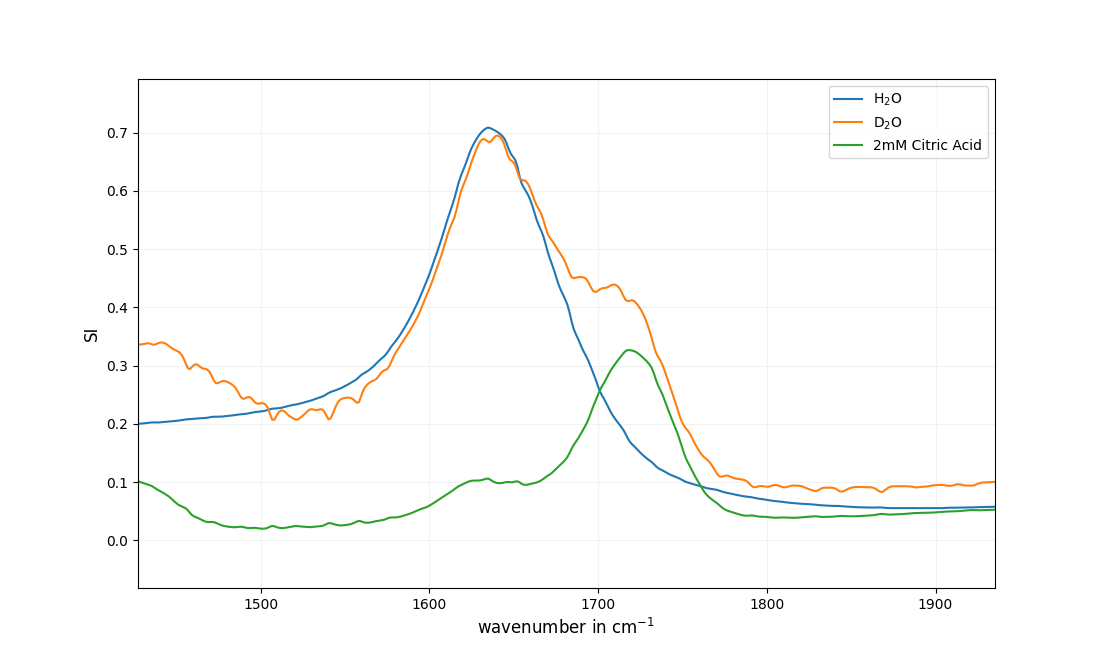
\includegraphics[scale=0.65]{water_citricacid_upclose.png}
			\caption{Infrarotspektrum von Wasser, Deuteriumoxid und 2mM Citronensäure in Wasser. Die Extrema in dem Bereich von Wasser und Deuteriumoxid überlappen mit dem Peak von Citronensäure.}
			\label{fig:water_citricacid}
		\end{figure}
		
		
		\begin{figure}[H]
			\centering
			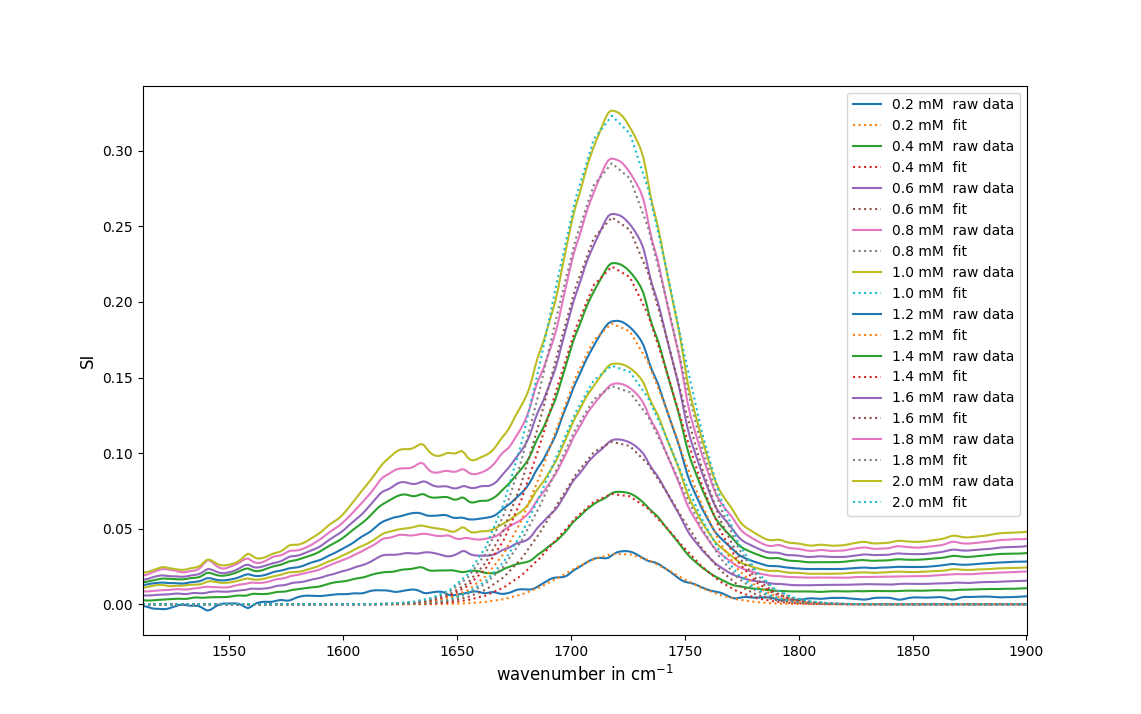
\includegraphics[scale=0.60]{Standardcurve_citricacid_fit.png}
			\caption{Infrarotspektrum der Verdünnungsreihe von Citronensäure in Wasser und der gaussche Fit des Maxima.}
			\label{fig:IR_Standardcurve}
		\end{figure}
	
		\subsubsection{Standardreihe Citronensäure}
			\begin{table}[H]
				\centering
				\caption{Pipettierschema der Standardreihe von Citronensäure in H$_2$O. Die molare Konzentration der Stammlösung beträgt 2mM in Wasser.}
				\label{tab:pipettierschema Standardreihe}
				\begin{tabular}{ccc}
					\toprule
					c(Citronensäure) in mM &V(2mM Citronensäure) in mL & V(H$_2$O in mL)\\
					\midrule
					2.0 & 2.0 & 0.0\\
					1.8 & 1.8 & 0.2\\
					1.6 & 1.6 & 0.4 \\
					1.4 & 1.4 & 0.6 \\
					1.2 & 1.2 & 0.8\\
					1.0 & 1.0 & 1.0 \\
					0.8 & 0.8 & 1.2\\
					0.6 & 0.6 & 1.4\\
					0.4 & 0.4 & 1.6 \\
					0.2 & 0.2 & 1.8 \\
					0.0 & 0.0 & 2.0\\
					\bottomrule
				\end{tabular}
			\end{table}	
	
	\addcontentsline{toc}{section}{References}
	\bibliographystyle{plainurl}
	\nocite{*}
	\bibliography{Literatur}
	\newpage
	
	
\end{document}